\documentclass[12pt,a4paper]{article}
\usepackage[utf8]{inputenc}
\usepackage[catalan]{babel}
\usepackage{graphicx}
\usepackage{geometry}
\usepackage{fancyhdr}
\usepackage{tabularx}
\usepackage{amsmath}
\usepackage{tikz}
\usepackage{tcolorbox}

% MARGES I CAPÇALERA
\geometry{top=3.5cm, bottom=2.5cm, left=2cm, right=2cm, headheight=2.5cm}

\pagestyle{fancy}
\fancyhf{}
% Assegura't de tenir els logos a la mateixa carpeta, o comenta aquestes línies per provar-ho
\fancyhead[L]{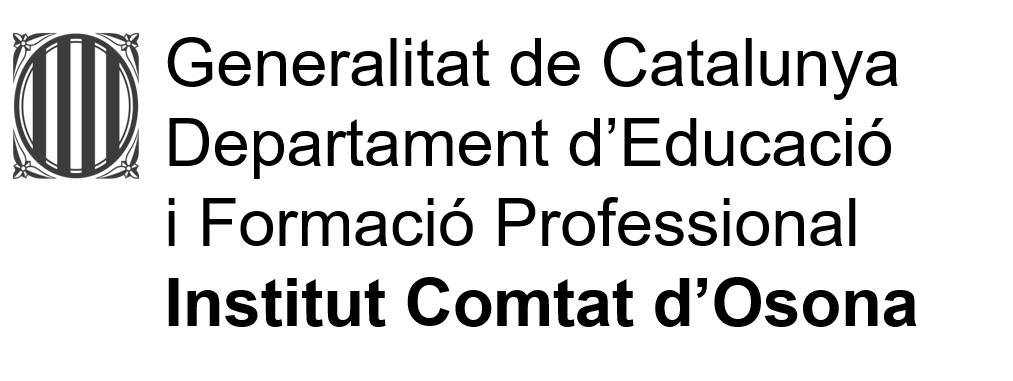
\includegraphics[height=1.5cm]{Logo_Departament.png}} 
\fancyhead[R]{
\includegraphics[height=1.5cm]{Logo_Institut.png}}
\fancyfoot[C]{Fitxa 2: Introducció a la Trigonometria - Pàgina \thepage}

\begin{document}

% --- CAPÇALERA D'IDENTIFICACIÓ ---
\begingroup
\renewcommand{\arraystretch}{1.8}
\begin{tabularx}{\textwidth}{|X|p{4cm}|}
    \hline
    \textbf{Nom i cognoms:} & \textbf{Grup:} \\ \hline
    \textbf{Activitat:} Fitxa 2. Sinus, Cosinus i Tangent & \textbf{Data:} \\ \hline
\end{tabularx}
\endgroup

\vspace{0.4cm}

\begin{tcolorbox}[colback=blue!5,colframe=blue!75,title=Recorda: Els noms dels costats]
En un triangle rectangle, els costats reben noms segons on es troben respecte a l'angle $\alpha$:
\begin{itemize}
    \item \textbf{Hipotenusa (H):} El costat més llarg (sempre davant de l'angle recte).
    \item \textbf{Catet Oposat (CO):} El catet que \textbf{no toca} l'angle $\alpha$ (està al davant).
    \item \textbf{Catet Contigu o Adjacent (CA):} El catet que \textbf{toca} l'angle $\alpha$ (en forma part).
\end{itemize}
\end{tcolorbox}

\section*{Pas 1: Identifica els costats (Repetició)}
\textbf{Exercici 1.} Escriu \textbf{Hipotenusa}, \textbf{Oposat} o \textbf{Adjacent} sobre la línia de punts de cada costat, segons l'angle marcat ($\alpha$). \textit{Vigila, el triangle pot estar girat!}

\vspace{0.3cm}
\begin{tabularx}{\textwidth}{@{} X X X @{}}
    a) \begin{tikzpicture}[scale=0.9]
        \draw[thick] (0,0) -- (3,0) -- (0,2) -- cycle;
        \draw (0.3,0) -- (0.3,0.3) -- (0,0.3); % Angle recte
        \draw (2.2,0) arc (180:146:0.8); % Arc més gran
        \node at (2.4,0.2) {$\alpha$}; 
        \node at (1.5,-0.4) {\dots\dots}; \node at (-0.6,1) {\dots\dots}; \node at (1.8,1.3) {\dots\dots};
    \end{tikzpicture} &
    b) \begin{tikzpicture}[scale=0.9]
        \draw[thick] (0,0) -- (0,2) -- (3,2) -- cycle;
        \draw (0,1.7) -- (0.3,1.7) -- (0.3,2); % Angle recte
        \draw (2.2,2) arc (180:213:0.8); % Arc més gran
        \node at (2.43,1.83) {$\alpha$}; 
        \node at (1.5,2.4) {\dots\dots}; \node at (-0.6,1) {\dots\dots}; \node at (1.8,0.7) {\dots\dots};
    \end{tikzpicture} &
    c) \begin{tikzpicture}[scale=0.9, rotate=90]
        \draw[thick] (0,0) -- (3,0) -- (3,2) -- cycle;
        \draw (2.7,0) -- (2.7,0.3) -- (3,0.3); % Angle recte
        \draw (0.8,0) arc (0:33:0.8); % Arc més gran
        \node at (0.6,0.2) {$\alpha$}; 
        \node at (1.5,-0.4) {\dots\dots}; \node at (3.6,1) {\dots\dots}; \node at (1.2,1.3) {\dots\dots};
    \end{tikzpicture}
\end{tabularx}

\vspace{0.6cm}

\begin{tcolorbox}[colback=orange!5,colframe=orange!75,title=La Regla Màgica: SOH CAH TOA]
Aquesta regla t'ajudarà a recordar les tres fórmules (A = Adjacent o Contigu):
\begin{center}
    \Large \textbf{S}in $\alpha = \frac{\mathbf{O}}{\mathbf{H}}$ \qquad \textbf{C}os $\alpha = \frac{\mathbf{A}}{\mathbf{H}}$ \qquad \textbf{T}an $\alpha = \frac{\mathbf{O}}{\mathbf{A}}$
\end{center}
\end{tcolorbox}

\section*{Pas 2: Calcula les raons trigonomètriques}
\textbf{Exercici 2.} Per a cada triangle:
1) Mesura l'angle $\alpha$ amb el teu transportador d'angles.
2) Omple les fraccions amb els costats correctes i calcula el decimal amb la calculadora.

\vspace{0.4cm}

% Triangle 1
\noindent\begin{minipage}{0.4\textwidth}
    \textbf{a)} \\
    \begin{tikzpicture}[scale=0.8]
        \draw[thick] (0,0) -- (4,0) node[midway,below]{$4$} -- (0,3) node[midway,above right]{$5$} -- cycle node[midway,left]{$3$};
        \draw (0.3,0) -- (0.3,0.3) -- (0,0.3);
        \draw (3.2,0) arc (180:143:0.8);
        \node at (3.47,0.2) {$\alpha$}; 
    \end{tikzpicture}
\end{minipage}
\begin{minipage}{0.55\textwidth}
    Mesura amb transportador: $\alpha \approx$ \makebox[1.5cm]{\hrulefill}$^\circ$ \\[0.3cm]
    $\sin \alpha = \dfrac{\text{CO}}{\text{H}} = \dfrac{\hspace{1cm}}{\hspace{1cm}} = \dots\dots\dots$ \\[0.4cm]
    $\cos \alpha = \dfrac{\text{CC}}{\text{H}} = \dfrac{\hspace{1cm}}{\hspace{1cm}}  = \dots\dots\dots$ \\[0.4cm]
    $\tan \alpha = \dfrac{\text{CO}}{\text{CC}} = \dfrac{\hspace{1cm}}{\hspace{1cm}} = \dots\dots\dots$
\end{minipage}

\vspace{0.8cm}

% Triangle 2
\noindent\begin{minipage}{0.4\textwidth}
    \textbf{b)} \\
    \begin{tikzpicture}[scale=0.6]
        \draw[thick] (0,0) -- (5,0) node[midway,below]{$5$} -- (0,12) node[midway,above right]{$13$} -- cycle node[midway,left]{$12$};
        \draw (0.4,0) -- (0.4,0.4) -- (0,0.4);
        \draw (4.2,0) arc (180:112:0.8);
        \node at (4.52,0.35) {$\alpha$}; 
    \end{tikzpicture}
\end{minipage}
\begin{minipage}{0.55\textwidth}
    Mesura amb transportador: $\alpha \approx$ \makebox[1.5cm]{\hrulefill}$^\circ$ \\[0.3cm]
    $\sin \alpha = \dfrac{\hspace{1cm}}{\hspace{1cm}} = \dots\dots\dots$ \\[0.4cm]
    $\cos \alpha = \dfrac{\hspace{1cm}}{\hspace{1cm}} = \dots\dots\dots$ \\[0.4cm]
    $\tan \alpha = \dfrac{\hspace{1cm}}{\hspace{1cm}} = \dots\dots\dots$
\end{minipage}

\newpage

% Triangle 3
\noindent\begin{minipage}{0.4\textwidth}
    \textbf{c)} \\
    \begin{tikzpicture}[scale=0.7]
        \draw[thick] (0,0) -- (8,0) node[midway,below]{$8$} -- (0,6) node[midway,above right]{$10$} -- cycle node[midway,left]{$6$};
        \draw (0.4,0) -- (0.4,0.4) -- (0,0.4);
        \draw (0,4.8) arc (-90:-37:1.2);
        \node at (0.4,4.2) {$\alpha$}; 
    \end{tikzpicture}
\end{minipage}
\begin{minipage}{0.55\textwidth}
    Mesura amb transportador: $\alpha \approx$ \makebox[1.5cm]{\hrulefill}$^\circ$ \\[0.3cm]
    $\sin \alpha = \dfrac{\text{CO}}{\text{H}} = \dfrac{\hspace{1cm}}{\hspace{1cm}} = \dots\dots\dots$ \\[0.4cm]
    $\cos \alpha = \dfrac{\text{CC}}{\text{H}} = \dfrac{\hspace{1cm}}{\hspace{1cm}}  = \dots\dots\dots$ \\[0.4cm]
    $\tan \alpha = \dfrac{\text{CO}}{\text{CC}} = \dfrac{\hspace{1cm}}{\hspace{1cm}} = \dots\dots\dots$
\end{minipage}

\vspace{0.8cm}

% Triangle 4 i comprovació
\noindent\begin{minipage}{0.4\textwidth}
    \textbf{d)} \\
    \begin{tikzpicture}[scale=0.4]
        \draw[thick] (0,0) -- (15,0) node[midway,below]{$15$} -- (0,8) node[midway,above right]{$17$} -- cycle node[midway,left]{$8$};
        \draw (0.6,0) -- (0.6,0.6) -- (0,0.6);
        \draw (12.5,0) arc (180:152:2.5);
        \node at (13,0.5) {$\alpha$}; 
    \end{tikzpicture}
\end{minipage}
\begin{minipage}{0.55\textwidth}
    Mesura amb transportador: $\alpha \approx$ \makebox[1.5cm]{\hrulefill}$^\circ$ \\[0.3cm]
    $\sin \alpha = \dfrac{\text{CO}}{\text{H}} = \dfrac{\hspace{1cm}}{\hspace{1cm}} = \dots\dots\dots$ \\[0.4cm]
    $\cos \alpha = \dfrac{\text{CC}}{\text{H}} = \dfrac{\hspace{1cm}}{\hspace{1cm}}  = \dots\dots\dots$ \\[0.4cm]
    $\tan \alpha = \dfrac{\text{CO}}{\text{CC}} = \dfrac{\hspace{1cm}}{\hspace{1cm}} = \dots\dots\dots$
\end{minipage}

\vspace{0.3cm}
\begin{tcolorbox}[colback=yellow!10,colframe=yellow!60!black,title=La màgia de desfer: \textbf{arcsin, arccos, arctan}]
Ara utilitzarem la calculadora per descobrir l'angle exacte a partir dels resultats anteriors (utilitza la tecla \texttt{SHIFT} o \texttt{INV} i després $\sin, \cos$ o $\tan$). Fes-ho per cada exercici.:
\begin{itemize}
    \item Si $\sin \alpha = \dots\dots\dots \longrightarrow \arcsin(\dots\dots\dots) = \makebox[2cm]{\hrulefill}^\circ$
    \item Si $\cos \alpha = \dots\dots\dots \longrightarrow \arccos(\dots\dots\dots) = \makebox[2cm]{\hrulefill}^\circ$
    \item Si $\tan \alpha = \dots\dots\dots \longrightarrow \arctan(\dots\dots\dots) = \makebox[2cm]{\hrulefill}^\circ$
\end{itemize}
\textbf{Reflexiona:} Et dona el mateix angle en tots tres casos? Coincideix amb el que havies mesurat a ull amb el transportador? \makebox[5cm]{\hrulefill}
\end{tcolorbox}

\vspace{0.8cm}

\newpage

\section*{Pas 3: Descobrint l'angle amagat}
\textbf{Exercici 3.} En aquests triangles només et donem \textbf{dos costats}. Fixa't quins costats són (CO, CC o H), tria la raó correcta (sin, cos o tan) i fes servir la calculadora ($\arcsin, \arccos, \arctan$) per trobar l'angle $\alpha$.

\vspace{0.5cm}

\begin{tabularx}{\textwidth}{@{} X X X @{}}
    % Exercici 1 (Sinus)
    \begin{tikzpicture}[scale=0.6]
        \draw[thick] (0,0) -- (3,0) -- (0,4) node[midway,right]{$8$} -- cycle node[midway,left]{$6$};
        \draw (0.4,0) -- (0.4,0.4) -- (0,0.4);
        \draw (2.2,0) arc (180:127:0.8);
        \node at (2,0.3) {$\alpha$}; 
    \end{tikzpicture} &
    % Exercici 2 (Tangent)
    \begin{tikzpicture}[scale=0.6]
        \draw[thick] (0,0) -- (4,0) node[midway,below]{$10$} -- (0,3) -- cycle node[midway,left]{$5$};
        \draw (0.4,0) -- (0.4,0.4) -- (0,0.4);
        \draw (3.2,0) arc (180:143:0.8);
        \node at (2.7,0.2) {$\alpha$}; 
    \end{tikzpicture} &
    % Exercici 3 (Cosinus)
    \begin{tikzpicture}[scale=0.6]
        \draw[thick] (0,0) -- (4,0) node[midway,below]{$5$} -- (0,4) node[midway,right]{$10$} -- cycle;
        \draw (0.4,0) -- (0.4,0.4) -- (0,0.4);
        \draw (3.2,0) arc (180:135:0.8);
        \node at (2.5,0.2) {$\alpha$}; 
    \end{tikzpicture} \\
    Tinc: \makebox[2cm]{\hrulefill} & Tinc: \makebox[2cm]{\hrulefill} & Tinc: \makebox[2cm]{\hrulefill} \\
    Faig servir: \makebox[1.5cm]{\hrulefill} & Faig servir: \makebox[1.5cm]{\hrulefill} & Faig servir: \makebox[1.5cm]{\hrulefill} \\ 
    \vspace{1cm} $\alpha = \dots\dots\dots^\circ$ & \vspace{1cm}  $\alpha = \dots\dots\dots^\circ$ & \vspace{1cm}  $\alpha = \dots\dots\dots^\circ$ \\[1cm]
    \vspace{1cm} \\
    % Exercici 4 (Tangent)
    \begin{tikzpicture}[scale=0.6]
        \draw[thick] (0,0) -- (3,0) node[midway,below]{$6$} -- (0,4) node[midway,right]{$8$} -- cycle;
        \draw (0.4,0) -- (0.4,0.4) -- (0,0.4);
        \draw (0,3.2) arc (-90:-53:0.8);
        \node at (0.4,2.8) {$\alpha$}; 
    \end{tikzpicture} &
    % Exercici 5 (Sinus)
    \begin{tikzpicture}[scale=0.6]
        \draw[thick] (0,0) -- (3,0) node[midway,below]{$6$} -- (0,4) -- cycle node[midway,left]{$10$};
        \draw (0.4,0) -- (0.4,0.4) -- (0,0.4);
        \draw (0,3.2) arc (-90:-53:0.8);
        \node at (0.4,2.8) {$\alpha$}; 
    \end{tikzpicture} &
    % Exercici 6 (Cosinus)
    \begin{tikzpicture}[scale=0.6]
        \draw[thick] (0,0) -- (3,0) -- (0,4) node[midway,right]{$12$} -- cycle node[midway,left]{$6$};
        \draw (0.4,0) -- (0.4,0.4) -- (0,0.4);
        \draw (0,3.2) arc (-90:-53:0.8);
        \node at (0.4,2.8) {$\alpha$}; 
    \end{tikzpicture} \\
    Tinc: \makebox[2cm]{\hrulefill} & Tinc: \makebox[2cm]{\hrulefill} & Tinc: \makebox[2cm]{\hrulefill} \\
    Faig servir: \makebox[1.5cm]{\hrulefill} & Faig servir: \makebox[1.5cm]{\hrulefill} & Faig servir: \makebox[1.5cm]{\hrulefill} \\
    \vspace{1cm} $\alpha = \dots\dots\dots^\circ$ & \vspace{1cm}  $\alpha = \dots\dots\dots^\circ$ & \vspace{1cm}  $\alpha = \dots\dots\dots^\circ$ \\
\end{tabularx}

\end{document}